%!TEX root = Manuscript.tex

\chapter{Use case of matching guided by 2D similarity transformation model}
\label{chap:appendix3}

\section{Dataset}

\begin{figure*}[htbp]
	\begin{center}
		\subfigure[Image 1]{
			\begin{minipage}[t]{0.31\linewidth}
				\centering
				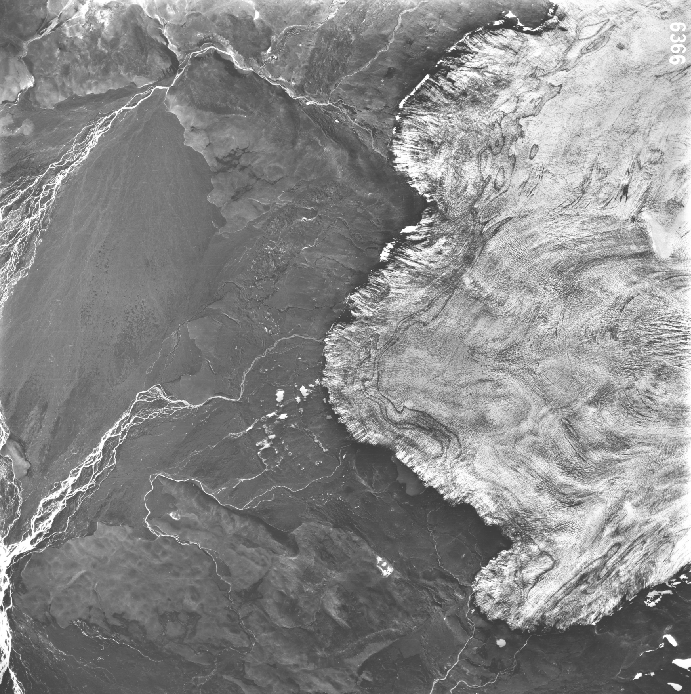
\includegraphics[width=4.3cm]{images/appendix3/3-6366_crp_8Bits_Zoom8.png}
			\end{minipage}%
		}
		\subfigure[Image 2]{
	\begin{minipage}[t]{0.31\linewidth}
		\centering
		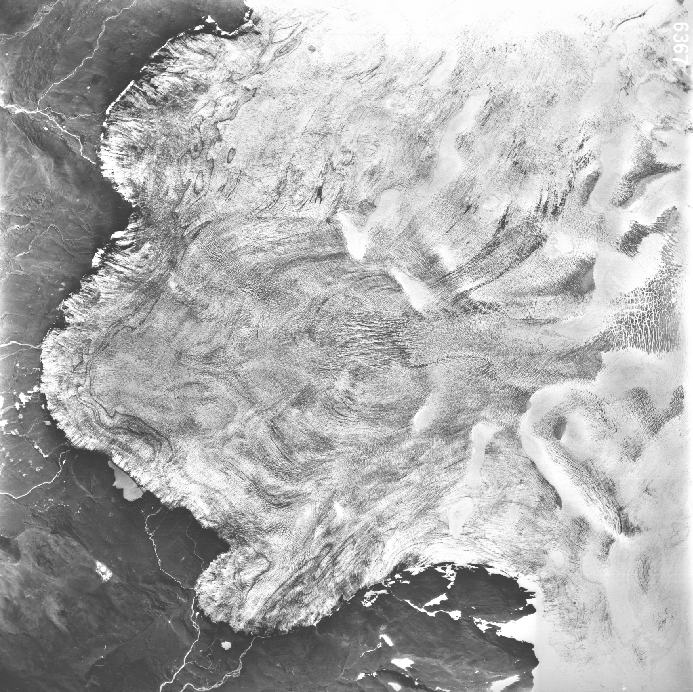
\includegraphics[width=4.3cm]{images/appendix3/3-6367_crp_8Bits_Zoom8.png}
	\end{minipage}%
}
		\subfigure[Image 3]{
	\begin{minipage}[t]{0.31\linewidth}
		\centering
		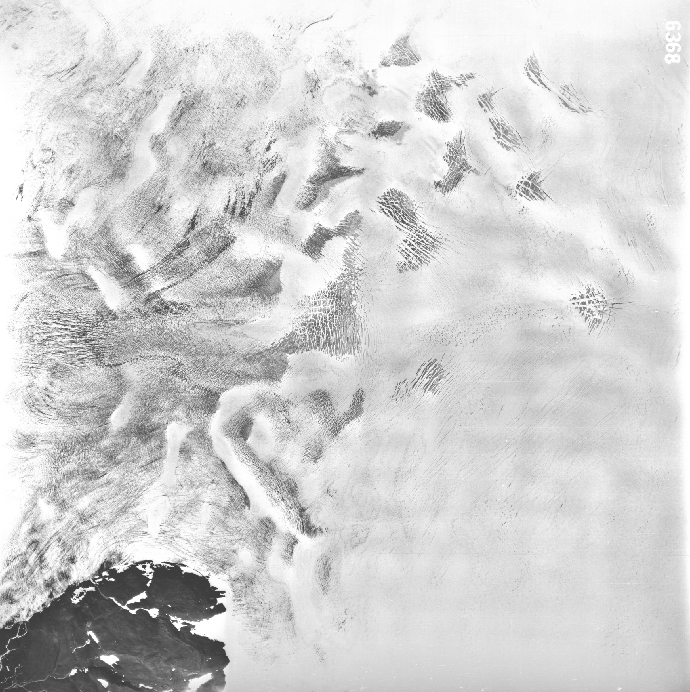
\includegraphics[width=4.3cm]{images/appendix3/3-6368_crp_8Bits_Zoom8.png}
	\end{minipage}%
}
		\subfigure[Image 1]{
	\begin{minipage}[t]{0.31\linewidth}
		\centering
		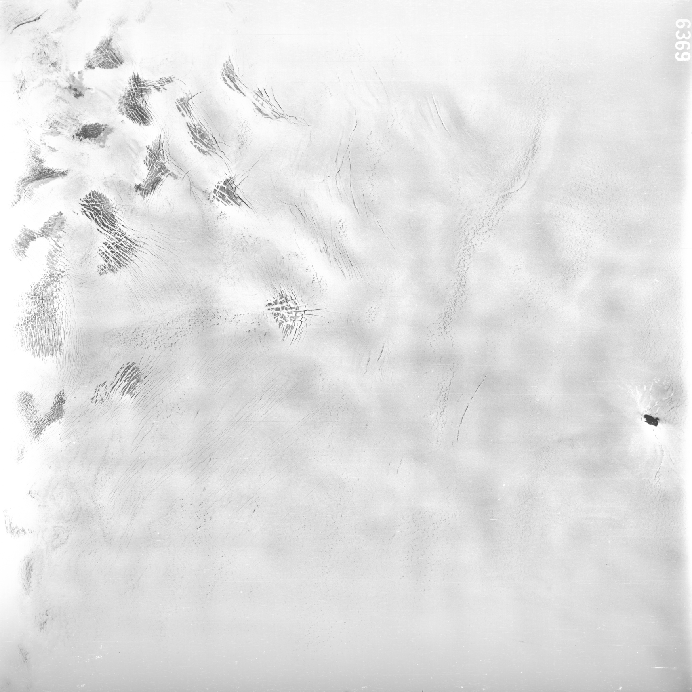
\includegraphics[width=4.3cm]{images/appendix3/3-6369_crp_8Bits_Zoom8.png}
	\end{minipage}%
}
\subfigure[Image 2]{
	\begin{minipage}[t]{0.31\linewidth}
		\centering
		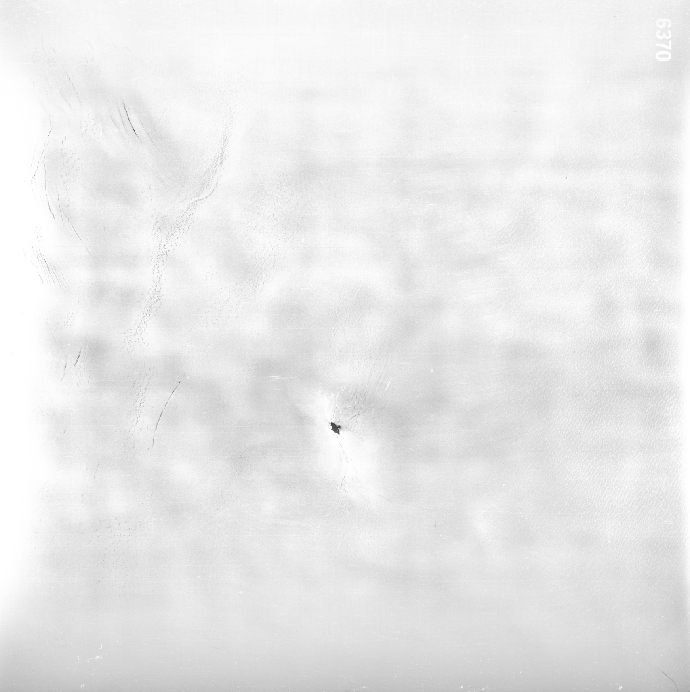
\includegraphics[width=4.3cm]{images/appendix3/3-6370_crp_8Bits_Zoom8.png}
	\end{minipage}%
}
\subfigure[Image 3]{
	\begin{minipage}[t]{0.31\linewidth}
		\centering
		
\includegraphics[width=4.3cm]{images/appendix3/3-6371_crp_8Bits_Zoom8.png}
	\end{minipage}%
}
		\caption{Dataset}
		\label{Match result}
	\end{center}
\end{figure*} 
